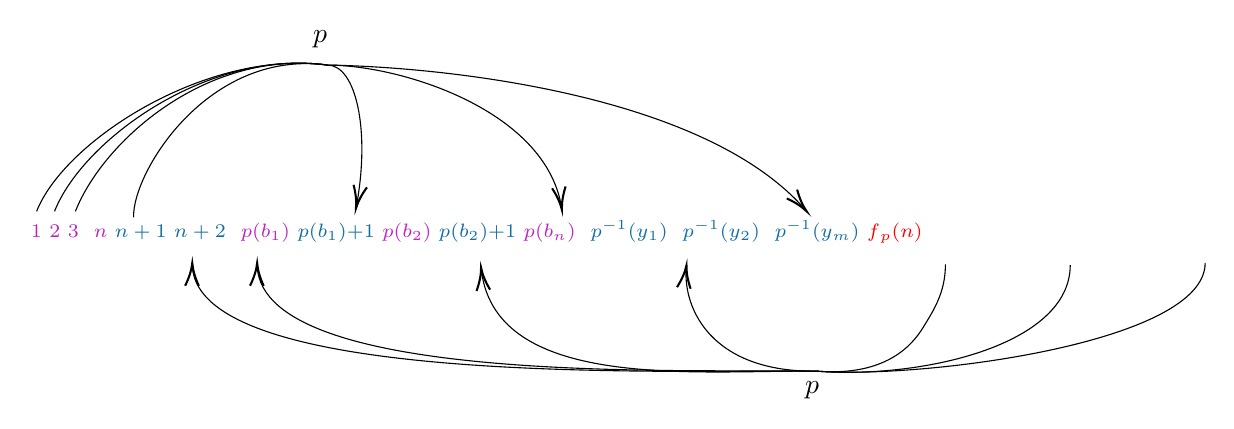
\begin{tikzpicture}[x=0.75pt,y=0.75pt,yscale=-1,xscale=1]
    %uncomment if require: \path (0,300); %set diagram left start at 0, and has height of 300
    
    %Curve Lines [id:da869685567152708] 
    \draw    (45,149.62) .. controls (58.66,115.11) and (127.68,71.25) .. (185.2,79.16) ;
    %Curve Lines [id:da45348245378320906] 
    \draw    (53.63,149.62) .. controls (67.29,115.11) and (127.68,71.25) .. (185.2,79.16) ;
    %Curve Lines [id:da15163922233603622] 
    \draw    (63.69,149.62) .. controls (77.35,115.11) and (127.68,71.25) .. (185.2,79.16) ;
    %Curve Lines [id:da4266797108919014] 
    \draw    (185.2,79.16) .. controls (198.66,79.16) and (205.84,109.86) .. (199.18,146.51) ;
    \draw [shift={(198.86,148.19)}, rotate = 280.89] [color={rgb, 255:red, 0; green, 0; blue, 0 }  ][line width=0.75]    (10.93,-3.29) .. controls (6.95,-1.4) and (3.31,-0.3) .. (0,0) .. controls (3.31,0.3) and (6.95,1.4) .. (10.93,3.29)   ;
    %Curve Lines [id:da09212583179865697] 
    \draw    (185.2,79.16) .. controls (220.79,79.16) and (290.21,101.01) .. (297.87,147.49) ;
    \draw [shift={(298.09,148.91)}, rotate = 262.23] [color={rgb, 255:red, 0; green, 0; blue, 0 }  ][line width=0.75]    (10.93,-3.29) .. controls (6.95,-1.4) and (3.31,-0.3) .. (0,0) .. controls (3.31,0.3) and (6.95,1.4) .. (10.93,3.29)   ;
    %Curve Lines [id:da05325802271682478] 
    \draw    (185.2,79.16) .. controls (236.71,79.88) and (365.81,91.98) .. (415.26,148.76) ;
    \draw [shift={(416,149.62)}, rotate = 229.64] [color={rgb, 255:red, 0; green, 0; blue, 0 }  ][line width=0.75]    (10.93,-3.29) .. controls (6.95,-1.4) and (3.31,-0.3) .. (0,0) .. controls (3.31,0.3) and (6.95,1.4) .. (10.93,3.29)   ;
    %Curve Lines [id:da5942864735244722] 
    \draw    (91.73,152.5) .. controls (91.02,130.93) and (127.68,71.25) .. (185.2,79.16) ;
    %Curve Lines [id:da7086658294610786] 
    \draw    (482.86,175.16) .. controls (482.86,188.43) and (477.47,196.87) .. (472.13,205.55) .. controls (466.79,214.23) and (454.11,229.1) .. (421.35,226.65) ;
    %Curve Lines [id:da3029725893649463] 
    \draw    (543,175.5) .. controls (543,214.19) and (471.2,230.37) .. (421.35,226.65) ;
    %Curve Lines [id:da8956250403734121] 
    \draw    (608,174.5) .. controls (608,213.19) and (471.2,230.37) .. (421.35,226.65) ;
    %Curve Lines [id:da9885601314892218] 
    \draw    (421.35,226.65) .. controls (355.05,225.91) and (123.94,234.66) .. (120.05,176.35) ;
    \draw [shift={(120,174.56)}, rotate = 90.71] [color={rgb, 255:red, 0; green, 0; blue, 0 }  ][line width=0.75]    (10.93,-3.29) .. controls (6.95,-1.4) and (3.31,-0.3) .. (0,0) .. controls (3.31,0.3) and (6.95,1.4) .. (10.93,3.29)   ;
    %Curve Lines [id:da36001142635919847] 
    \draw    (421.35,226.65) .. controls (364.63,225.18) and (154.76,234.64) .. (151.29,176.35) ;
    \draw [shift={(151.25,174.56)}, rotate = 90.71] [color={rgb, 255:red, 0; green, 0; blue, 0 }  ][line width=0.75]    (10.93,-3.29) .. controls (6.95,-1.4) and (3.31,-0.3) .. (0,0) .. controls (3.31,0.3) and (6.95,1.4) .. (10.93,3.29)   ;
    %Curve Lines [id:da06532490587760609] 
    \draw    (421.35,226.65) .. controls (365.37,225.91) and (267.08,236.85) .. (259.35,178.58) ;
    \draw [shift={(259.14,176.8)}, rotate = 84.36] [color={rgb, 255:red, 0; green, 0; blue, 0 }  ][line width=0.75]    (10.93,-3.29) .. controls (6.95,-1.4) and (3.31,-0.3) .. (0,0) .. controls (3.31,0.3) and (6.95,1.4) .. (10.93,3.29)   ;
    %Curve Lines [id:da921688325305408] 
    \draw    (421.35,226.65) .. controls (370.11,227.37) and (356.67,196.59) .. (357.94,177.42) ;
    \draw [shift={(358.1,175.68)}, rotate = 96.71] [color={rgb, 255:red, 0; green, 0; blue, 0 }  ][line width=0.75]    (10.93,-3.29) .. controls (6.95,-1.4) and (3.31,-0.3) .. (0,0) .. controls (3.31,0.3) and (6.95,1.4) .. (10.93,3.29)   ;
    
    % Text Node
    \draw (40.96,152.68) node [anchor=north west][inner sep=0.75pt]  [font=\scriptsize]  {$\textcolor[rgb]{0.74,0.14,0.75}{1\ 2\ 3\ \dotsc \ n} \ \boxed{\textcolor[rgb]{0.08,0.43,0.64}{n+1\ n+2\ \dotsc }}\textcolor[rgb]{0.74,0.14,0.75}{\ p}\textcolor[rgb]{0.74,0.14,0.75}{( b}\textcolor[rgb]{0.74,0.14,0.75}{_{1}}\textcolor[rgb]{0.74,0.14,0.75}{)} \ \boxed{\textcolor[rgb]{0.08,0.43,0.64}{p}\textcolor[rgb]{0.08,0.43,0.64}{( b}\textcolor[rgb]{0.08,0.43,0.64}{_{1}}\textcolor[rgb]{0.08,0.43,0.64}{)}\textcolor[rgb]{0.08,0.43,0.64}{+1\dotsc }} \ \textcolor[rgb]{0.74,0.14,0.75}{p}\textcolor[rgb]{0.74,0.14,0.75}{( b}\textcolor[rgb]{0.74,0.14,0.75}{_{2}}\textcolor[rgb]{0.74,0.14,0.75}{)} \ \boxed{\textcolor[rgb]{0.08,0.43,0.64}{p}\textcolor[rgb]{0.08,0.43,0.64}{( b}\textcolor[rgb]{0.08,0.43,0.64}{_{2}}\textcolor[rgb]{0.08,0.43,0.64}{)}\textcolor[rgb]{0.08,0.43,0.64}{+1\dotsc }} \ \dotsc \textcolor[rgb]{0.74,0.14,0.75}{p}\textcolor[rgb]{0.74,0.14,0.75}{( b}\textcolor[rgb]{0.74,0.14,0.75}{_{n}}\textcolor[rgb]{0.74,0.14,0.75}{)} \ \dotsc \ \textcolor[rgb]{0.08,0.43,0.64}{p}\textcolor[rgb]{0.08,0.43,0.64}{^{-1}}\textcolor[rgb]{0.08,0.43,0.64}{(}\textcolor[rgb]{0.08,0.43,0.64}{y}\textcolor[rgb]{0.08,0.43,0.64}{_{1}}\textcolor[rgb]{0.08,0.43,0.64}{)}\textcolor[rgb]{0.08,0.43,0.64}{\ } \dotsc \textcolor[rgb]{0.08,0.43,0.64}{\ p}\textcolor[rgb]{0.08,0.43,0.64}{^{-1}}\textcolor[rgb]{0.08,0.43,0.64}{(}\textcolor[rgb]{0.08,0.43,0.64}{y}\textcolor[rgb]{0.08,0.43,0.64}{_{2}}\textcolor[rgb]{0.08,0.43,0.64}{)}\textcolor[rgb]{0.08,0.43,0.64}{\ } \dotsc \textcolor[rgb]{0.08,0.43,0.64}{\ p}\textcolor[rgb]{0.08,0.43,0.64}{^{-1}}\textcolor[rgb]{0.08,0.43,0.64}{(}\textcolor[rgb]{0.08,0.43,0.64}{y}\textcolor[rgb]{0.08,0.43,0.64}{_{m}}\textcolor[rgb]{0.08,0.43,0.64}{)} \ \textcolor[rgb]{1,0,0}{f}\textcolor[rgb]{1,0,0}{_{p}}\textcolor[rgb]{1,0,0}{(}\textcolor[rgb]{1,0,0}{n}\textcolor[rgb]{1,0,0}{)}$};
    % Text Node
    \draw (177,61.4) node [anchor=north west][inner sep=0.75pt]    {$p$};
    % Text Node
    \draw (414,230.4) node [anchor=north west][inner sep=0.75pt]    {$p$};
\end{tikzpicture}